\documentclass[11pt]{article}

%https://de.overleaf.com/latex/templates/chapter-review-notes/npqqbrvfkwqh

\usepackage[utf8]{inputenc}	% Para caracteres en español
\usepackage{amsmath,amsthm,amsfonts,amssymb,amscd}
\usepackage{multirow,booktabs}
\usepackage[table]{xcolor}
\usepackage{fullpage}
\usepackage{lastpage}
\usepackage{enumitem}
\usepackage{fancyhdr}
\usepackage{mathrsfs}
\usepackage{wrapfig}
\usepackage{setspace}
\usepackage{calc}
\usepackage{multicol}
\usepackage{cancel}
\usepackage[retainorgcmds]{IEEEtrantools}
\usepackage[margin=3cm]{geometry}
\usepackage{amsmath}
\newlength{\tabcont}
\setlength{\parindent}{0.0in}
\setlength{\parskip}{0.05in}
\usepackage{empheq}
\usepackage{framed}
\usepackage[most]{tcolorbox}
\usepackage{xcolor}
\usepackage{tikz, hyperref}

\colorlet{shadecolor}{orange!15}
\parindent 0in
\parskip 12pt
\geometry{margin=1in, headsep=0.25in}
\theoremstyle{definition}
\newtheorem{defn}{Definition}
\newtheorem{reg}{Rule}
\newtheorem{exer}{Exercise}
\newtheorem{note}{Note}

\newcommand\copyrighttext{%
  \footnotesize All documents, webpages, photographs and images are the property of or licensed by the authors, except where noted. Permission is required to copy, download, or use any text, photographs, or image files.}
\newcommand\copyrightnotice{%
\begin{tikzpicture}[remember picture,overlay]
\node[anchor=south,yshift=10pt] at (current page.south) {\fbox{\parbox{\dimexpr\textwidth-\fboxsep-\fboxrule\relax}{\copyrighttext}}};
\end{tikzpicture}%
}


\begin{document}
\setcounter{section}{0}
\title{Getting Ready}

\thispagestyle{empty}

\begin{center}
{\LARGE \bf Data Science for High School}\\
{\large Summer 2021\\
Haim Bar, HaiYing Wang, and Jun Yan\\Department of Statistics, University of Connecticut}
\end{center}
\section{Before We Begin...}
In this class, we will use the R language, and the RStudio integrated development environment (IDE). Before the first meeting, install the necessary software on your personal computer by executing the following instructions.
%\subsection{Installing R and Rstudio}
Go to the website of the Comprehensive R Archive Network \url{https://cran.r-project.org/} and download the latest version of R for your operating system (Windows, MacOS, or Linux). As of \today, the latest version is 4.0.4. Follow the installation instructions.

Next, go the Rstudio download website \url{https://rstudio.com/products/rstudio/download/} and get the Desktop version (open source license). As of \today, the version is 1.4.1106. Follow the installation instruction. An icon that looks like this: 
\includegraphics[scale=0.3]{RstudioLogo.png} will be on your computer's desktop. Double-click on this icon to start the R session. The Rstudio IDE will open, and look like this:

\begin{center}
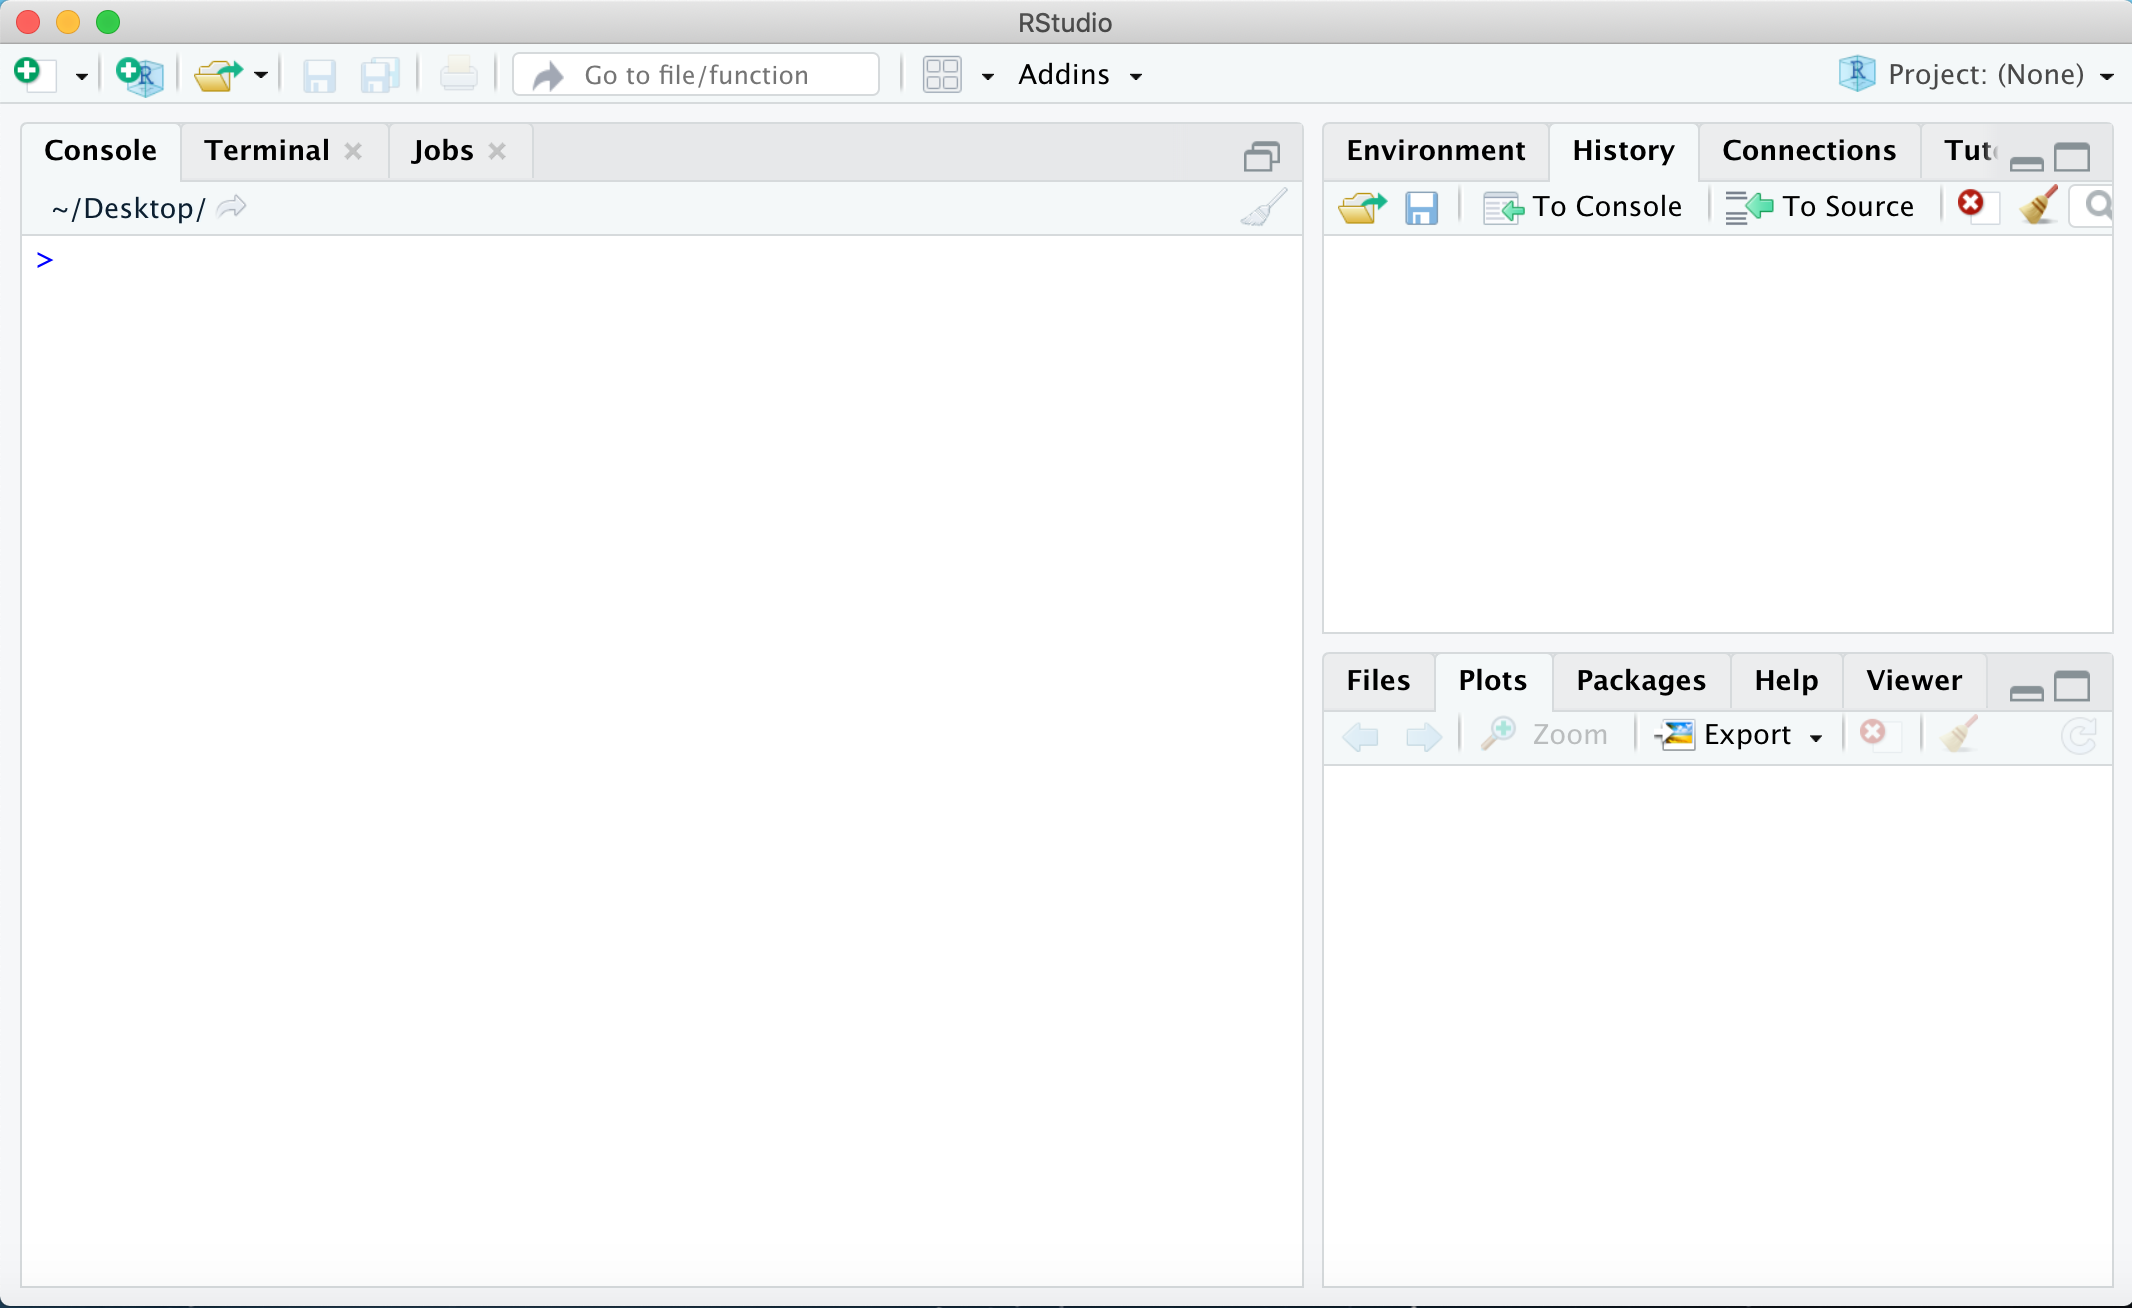
\includegraphics[scale=0.4]{RstudioMain.png}
\end{center}

The left-hand side of the screen contains the Console tab. Notice the $>$ sign (called the `prompt'). When you see this character, it means the R is ready for the next command. Put the cursor there, and then type\\
\begin{tcolorbox}[colback=gray!20,boxrule=0pt,frame hidden]
\begin{verbatim}
2+2
\end{verbatim}
\end{tcolorbox}
and hit Enter on the keyboard. You should get the following on the Console:
\begin{tcolorbox}[colback=gray!20,boxrule=0pt,frame hidden]
\begin{verbatim}
[1] 4
\end{verbatim}
\end{tcolorbox}

Notice the top-right part of the Rstudio window. You should see an `Environment' and a `History' tab. Click on History. Notice that your previous input appears there. Try entering another calculation or command and see that they appear in the session's history. For example, try entering the following (without the prompt sign)
 \begin{tcolorbox}[colback=gray!20,boxrule=0pt,frame hidden]
\begin{verbatim}
> 3^5
> date()
\end{verbatim}
\end{tcolorbox}

Click on the Environment tab. It should be empty when you start R for the first time. In the Console, type
\begin{tcolorbox}[colback=gray!20,boxrule=0pt,frame hidden]
\begin{verbatim}
> myFirstVariable <- factorial(5)
\end{verbatim}
\end{tcolorbox}
Notice that nothing was printed in the Console, but the Environment tab now contains a table with one row, with `myFirstVariable' appearing in the cell on the left, and its value (120) on the right. Any object appearing in the Environment tab is available to you throughout your R session, and you don't have to recalculate it. For example, you can try the following:
\begin{tcolorbox}[colback=gray!20,boxrule=0pt,frame hidden]
\begin{verbatim}
> myFirstVariable/6
\end{verbatim}
\end{tcolorbox}
The Console should now display 20.

The lower-right side of the IDE contains a file browser (the Files tab), information about installed packages (more about it later), and any plot generated during the R session. It also contains a Help tab, to obtain information about built-in functions.

Finally, before we move on to the next section, in the Rstudio top menu, click on File, then on New File, and then on R Script. Alternatively, you can click on little green `+' icon in the top-left part of the IDE. This will split the left side of the Rstudio IDE into two parts -- the lower part will contain the Console, and the top part will contain a tab labeled `Untitled1'. This is were you can enter R code which you will save to a permanent file, and re-use later.
For example, enter the following in the blank space in the Untitled1 tab:
\begin{tcolorbox}[colback=gray!20,boxrule=0pt,frame hidden]
\begin{verbatim}
# This is my first R program
cat('Hello, World!\n')
\end{verbatim}
\end{tcolorbox}
Then, click on File $>$ Save, and in the `Save As' box enter FirstProgram.R and click the Save button.
Notice that the tab name is now FirstProgram.R.

In that part of the window, there should now be a small button called Source. Click on it. The program will be executed and the output will be shown in the Console. You can also execute individual lines in the source code. Just put the cursor anywhere in that line, and click on the Run button (which is near the Source button.)

That's it. In the rest of these notes we will see more features of Rstudio, but you are now ready to start learning programming in R.

\section{Basic Operations in R}
In this course, much of the learning will be done by using simulated data, so let's start by learning how to generate data. The basic function to generate random data is \texttt{runif} which is used to draw random numbers, uniformly between 0 and 1. In the following example we create 10,000 random draws from a uniform distribution, keep these numbers in a variable called simData, and plot a histogram to show the distribution of the data we have generated. The \texttt{set.seed} function is used to ensure that every time we run this code, we will get the same set of random numbers. This is called \textit{reproducible code}. 
\begin{tcolorbox}[colback=gray!20,boxrule=0pt,frame hidden]
\begin{verbatim}
# Generate 10,000 points from a uniform distribution
set.seed(210313)
n <- 10000
simData <- runif(n)
hist(simData)
\end{verbatim}
\end{tcolorbox}
This will produce the following:
\begin{center}
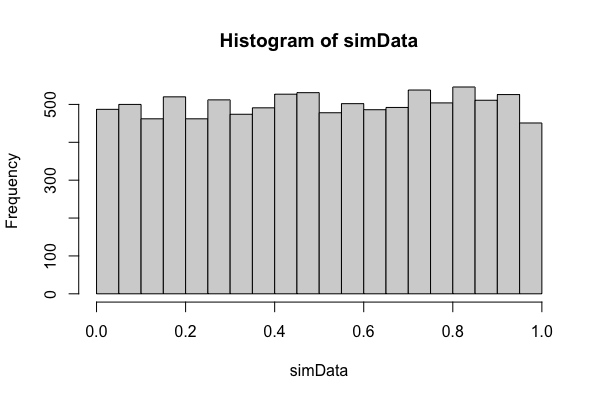
\includegraphics[scale=0.3]{Note01HistUnif.png}
\end{center}
From the range and the flatness of the histogram we can see that the generated data is indeed uniform on [0,1]. The \texttt{runif} function can be used to draw random numbers uniformly on any finite interval. For example, if we want our random numbers to be in the interval [1,5] we will run the following code:
\begin{tcolorbox}[colback=gray!20,boxrule=0pt,frame hidden]
\begin{verbatim}
simData <- runif(n, min=1, max=5)
\end{verbatim}
\end{tcolorbox}
Try it, and draw the histogram as in the previous example.



%Introduction to R and RNG descriptive/graph data summary: Haim
%    Summary statistics
%    Boxplots / Violin plots
%Homework ideas:
%    Generate data and summarize them


%\begin{shaded}
%\textbf{Some highlighted text}\newline
%The velocity at any point, \textit{P} (position, \textit{r}) is given by:
%\begin{equation}
%v = \omega\  x \ r
%\end{equation}
%\end{shaded}
%
%Consider an inertial reference frame (i.e not accelerating) which will be denoted S$_0$, and a accelerating reference frame, \textit{S} that has an acceleration of \textit{A}. 
%\begin{note}
%\textbf{Capital Letters refer to the accelerating reference frame \textit{S} while lowercase letters refer to the inertial reference frame S$_0$}
%\end{note}
%Picture a moving reference frame, \textit{S}, moving relative to S$_0$. Imagine in the the moving reference frame that a ball with mass, \textit{m} is being thrown. 
%In order to consider the motion of the ball, the motion must be first considered in the inertial reference frame. 
%\begin{equation}
%F = m\ddot{r_0}
%\end{equation}
%Where r$_0$ is the ball's position relative to S$_0$. 
%
%Now, by considering the motion of the ball in the accelerating frame, the ball position relative to \textit{S} is \textit{R}. (It's velocity is $\dot{R}$. 
%Thus, relating \textit{R} to $r_0$, we have: 
%\begin{equation}
%\dot{r_0} = \dot{R} + V
%\end{equation}
%Newton's second law for the inertial reference frame by differentiate and multiplying by mass is:
%\begin{equation}
%F_{\text{inertial}} = -mA = -m\ddot{R}
%\end{equation}
%\subsection{The Tides}
%\begin{shaded}
%\textbf{The Tidal Force} \newline
%\begin{equation}
%F_{tide} = -GM_mm(\frac{\hat{d}}{d^2}-\frac{\hat{d_0}}{d_0^2})
%\end{equation}
%Where:
%\begin{equation*}
%\begin{split}
%G = \text{Gravitational Constant} \\
%d = \text{Object's Position Relative to Moon} \\
%d_0 = \text{Earth's Center Relative to the moon}\\
%M_m = \text{Mass of the moon}
%\end{split}
%\end{equation*}
%\end{shaded}
%\newpage
%\subsection{The Angular Velocity Vector}
%The rest of the notes and the chapter will over reference frames that are rotating with respect to the inertial reference frame, so angular velocity has to be used. 
%\begin{defn}
%\textbf{Euler's Theorem} - The most general motion of any body relative to a fixed point \textit{O} is a rotation about some axis through \textit{O} To specify this rotation about a given point O, we only have to give the direction of the axis and the rate of rotation, or angular velocity $\omega$. Because this has a magnitude and direction, it is an obvious choice to write this rotation vector as $\omega$, the angular velocity vector. That is:
%\begin{equation}
%\omega = \omega\textbf{u}
%\end{equation}
%Where \textbf{u} is the unit vector
%\end{defn}
%\begin{shaded}
%\textbf{Vector Velocity}\newline
%The velocity at any point, \textit{P} (position, \textit{r}) is given by:
%\begin{equation}
%v = \omega\  x \ r
%\end{equation}
%\end{shaded}
%\subsection*{Addition of Angular Velocities}
%One can add angular velocities just like linear velocities. If body 3 is rotating at angular velocity $\omega_{32}$ relative to frame 2, and frame 2 is rotating at angular velocity $\omega_{21}$ relative to frame 1, then body 3 is rotating relative to frame 1 at angular velocity: 
%\begin{equation}
%\omega_{31} = \omega_{32} + \omega_{21}
%\end{equation}
%\subsection{Time Derivatives in Rotating Frames}
%If frame S has a angular velocity, $\Omega$ relative to S$_0$ then the time derivative of a single vector \textbf{Q} as seen in the two frames are related by:
%\begin{equation}
%(\frac{d\textbf{Q}}{dt})_{S_0} = (\frac{d\textbf{Q}}{dt})_{S} \ + \Omega \ x \ \textbf{Q}
%\end{equation}
%\subsection{Netwon's Second Law in a Rotating Frame}
%A particle in an inertial reference frame, S$_0$ obeys Newton's second law as we are use to:
%\begin{equation}
%m\frac{d^2r}{dt^2} = F
%\end{equation}
%Using the results from equation 8, the time derivative for a rotating frame with reference to an inertial frame can be given by:
%\begin{equation}
%(\frac{dr}{dt})_{S_0} = (\frac{dr}{dt})_s \ + \Omega \ x \ r
%\end{equation}
%By differentiation, Newton's second law becomes:
%\begin{equation}
%m\ddot{r} = F + 2m\dot{r} \ x \ \Omega \ + m(\Omega \ x \ r) \ x \ \Omega
%\end{equation}
%Where \textit{F} is the sum of all forces in the inertial reference frame. 
%\subsection{The Centrifugal Force}
%This is an inertial force in a rotating reference frame 
%\begin{equation}
%F_{\text{cf}} = m(\Omega \ x \ r) \ x \ \Omega
%\end{equation}
%\subsubsection*{Free-Fall Acceleration (Non-Vertical Gravity)}
%\begin{equation}
%F_{\text{eff}} = F_{\text{grav}} + F_{\text{cf}} = mg_0 + m\Omega^2R\sin(\theta)\hat{\rho}
%\end{equation}
%The acceleration due to the Centrifugal force is simply 
%\begin{equation}
%\begin{split}
%g = g_0 + \Omega^2R\sin(\theta)\hat{\rho} \\
%g_{\text{rad}} = g_0 - \Omega^2R\sin^2(\theta)  \\
%g_{\text{tan}} = \Omega^2R\sin(\theta)\cos(\theta)
%\end{split}
%\end{equation}
%The angle between g and its radial direction is:
%\begin{equation}
%\alpha \approx \frac{g_{\text{tan}}}{g_{\text{rad}}} 
%\end{equation}
%The maxium value at ($\theta$ = 45):
%\begin{equation}
%\alpha_{\text{max}} =  \frac{\Omega^2R}{2g_0}
%\end{equation}
%\subsection{Coriolis Force}
%The Coriolis Force is another inertial force in a rotating reference frame that an object experiences when it is moving. 
%\begin{equation}
%F_{\text{cor}} = 2m\dot{r} \ x \ \Omega = 2mv \ x \ \Omega
%\end{equation}
%The maximum acceleration, \textit{a} that the Coriolis force could produce acting by itself with \textit{v} perpendicular to $\Omega$ is:
%\begin{equation}
%a_{\text{max}} = 2v\Omega 
%\end{equation}
%\begin{shaded}
%\textbf{Direction of the Coriolis Force} \newline
%The Direction of the Coriolis force us always perpendicular to the velocity of the object (hence equation 17), and is given by the right hand rule. 
%\end{shaded}
%\newpage
%\subsection{Free Fall and the Coriolis Force}
%\begin{equation}
%m\ddot{r} = mg_0 + F_{\text{cf}} + F_{\text{cor}} 
%\end{equation}
%\subsection{The Foucault Pendulum}
%See chapter 9, Page 354. There is no need to recopy what is in the book here. 
%
\copyrightnotice

\end{document}
